\documentclass{article}

\usepackage{amsmath,amsthm,amssymb,amsfonts}
\newcommand{\R}{\ensuremath{\mathbb R}}
\usepackage{float}
\usepackage{graphicx}
\usepackage{breqn}
\usepackage[T1]{fontenc}
\usepackage{enumitem}


\usepackage{Sweave}
\begin{document}
\Sconcordance{concordance:Report.tex:Report.Rnw:%
1 32 1 1 0 39 1 1 3 2 0 3 1 3 0 1 4 5 0 1 2 1 1 1 3 2 0 2 1 21 0 5 1 4 %
0 1 2 8 1 1 2 1 0 2 1 1 2 3 1 4 0 1 2 2 1 1 2 1 0 2 1 1 2 5 1 4 0 1 2 5 %
1 1 3 2 0 2 1 1 3 1 0 2 1 1 3 1 0 2 1 1 3 1 0 2 1 1 3 1 0 2 1 3 0 1 2 %
66 1 1 3 2 0 3 1 3 0 1 2 1 1 1 20 19 0 2 2 1 0 3 1 3 0 1 2 4 1 1 3 2 0 %
1 1 1 2 5 0 1 2 11 1 1 3 2 0 2 1 1 7 9 0 1 2 24 1 1 3 2 0 3 1 4 0 1 2 4 %
1 1 3 12 0 1 2 17 1 1 3 2 0 1 1 4 0 1 2 2 1 1 3 2 0 2 1 11 0 1 2 2 1 1 %
3 2 0 1 1 4 0 1 2 10 1 1 3 17 0 1 2 13 1 1 3 2 0 1 1 4 0 1 2 3 1 1 3 2 %
0 2 1 15 0 1 2 1 1 1 3 2 0 1 1 4 0 1 2 1 1 1 3 2 0 2 2 2 1 4 0 1 2 3 1 %
1 3 2 0 1 1 14 0 2 1 4 0 1 2 10 1}


\title{COSC505 Project: Bitcoin Trading}
\author{Shima Amirsadri \and Deepak Kumar \and Shambhavi Singh} 
\date{\today}
\maketitle

\section{Introduction}
Bitcoin is one the famous worldwide cryptocurrency available in the market. First launched in 2009 by Satoshi Nakamoto as an open source software, it is a digital payment system which works without a central repository or single administrator. The system is peer to peer and the transactions takes place between users directly without any need of intermediary. It can also be exchanged for other currencies, products and services in most of countries. The historical bitcoin dataset contains the bitcoin trading market data from selected bitcoin exchanges. The data has been collected at an interval of one minute from Jan 2012 to Oct 2017. Bitcoin has seen a recent rise in popularity and its price has skyrocketed in the past 2 years. 

This report is divided into three major sections. Section\ref{secDataset} covers a brief description of our dataset. Section \ref{secModels} covers the models that were chosen to fit dataset for bitcoin in USD while section \ref{secARIMA} covers the forecasting of bitcoin values using an Autoregressive Integrated Moving Average(ARIMA) model.

\section{Dataset} \label{secDataset}
The dataset has been downloaded from Kaggle.com, and contains seven CSV files which stores the minute to minute updates for OHLC(Open, High, Low, Close), Volume in BTC and the corresponding currency, and weighted price of the bitcoin. The time of these transactions have been stored as timestamps according to Unix conventions while the data for timestamps with no trade or activity have been stored as NaNs.

The datasets are as follows:
\begin{itemize}
\item \textbf{coinbaseUSD\_1-min\_data\_2014-12-01\_to\_2017-10-20} stores the data obtained from the Coinbase bitcoin exchange in US Dollars from December 1st, 2014, to October 20, 2017.
\item \textbf{bitstampUSD\_1-min\_data\_2012-01-01\_to\_2017-10-20} stores the data obtained from the Bitstamp bitcoin exchange in US Dollars from January 1st, 2012, to October 20, 2017.
\item \textbf{coincheckJPY\_1-min\_data\_2014-10-31\_to\_2017-10-20} stores the data obtained from the Coincheck bitcoin exchange in Japanese Yen from October 31st, 2014, to October 20, 2017.
\item \textbf{btceUSD\_1-min\_data\_2012-01-01\_to\_2017-05-31} stores the data obtained from the BTC-e bitcoin exchange in US Dollars from January 1st, 2012, to May 31, 2017. Currently this exchange has been closed by US Justice Dept from July 26th, 2017.
\item \textbf{krakenEUR\_1-min\_data\_2014-01-08\_to\_2017-05-31}  stores the bitcoin trade data occurred between January 8, 2014 to May 31st, 2017 on Kraken exchange in Euros.
\item \textbf{krakenUSD\_1-min\_data\_2014-01-07\_to\_2017-05-31} stores the data obtained from the Kraken bitcoin exchange in US Dollars from January 7, 2014, to May 31st, 2017.
\item \textbf{btcnCNY\_1-min\_data\_2012-01-01\_to\_2017-05-31} stores the data obtained from the Chinese bitcoin market in Chinese Yuan from January 1st, 2012, to May 31, 2017.
\end{itemize}

\section{Model fitting} \label{secModels}
This section covers the models we tried to fit to our data.
%Please add the figures to their related positions according to the word document that I sent on Github for exponential model.
\subsection{Exponential Model Fitting}
Fitting an exponential model to the Bitcoin opening values
In order to fit an exponential model to the Bitcoin opening values, we have taken several steps. The first step is to clean the data. For this purpose, we removed all rows that contain missing values in their opening values. After that, using $qreference()$ method, we found out that our data is far from an exponential model because there are no similar patterns between our data and exponential reference plots.
\begin{Schunk}
\begin{Sinput}
> library(readr)
> qreference<-DAAG::qreference
> csv<-read_csv('bitstampUSD_1-min_data_2012-01-01_to_2017-10-20.csv')
> csv2<-csv[complete.cases(csv), ]
> open<-csv2$Open
\end{Sinput}
\end{Schunk}
\begin{Schunk}
\begin{Sinput}
> # Plotting qrefrence plots for checking if our data follows an exponential model
> qreference(open, xlab=" ",distribution = function(x) qexp(x, rate = 1/mean(open)) )
\end{Sinput}
\end{Schunk}
\newpage
\begin{figure}[H]
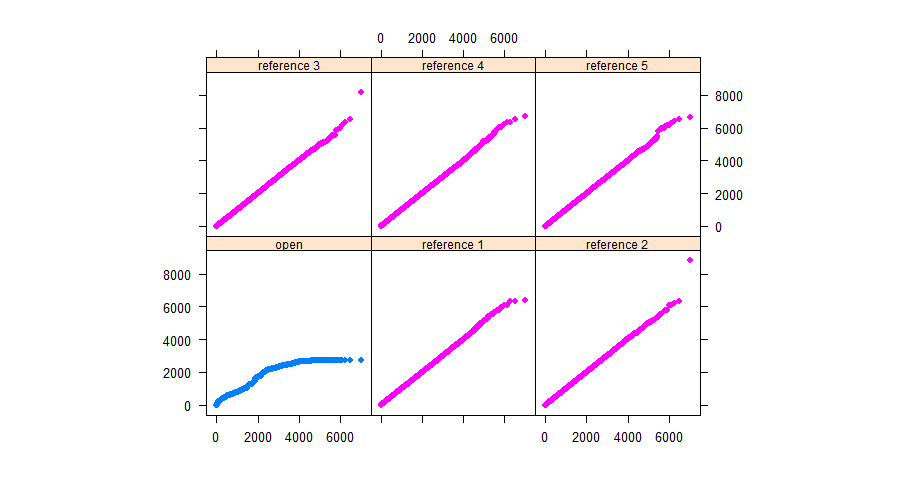
\includegraphics[width=1.1\textwidth]{qqref.png}
\end{figure}

In the next step, we fitted an exponential model to our data and then plotted it. For doing that, we fitted the linear model of log of the opening values, which is the same as fitting an exponential model of timestamp against opening values. From the plot, we realized that the trend of the Bitcoin opening values does not follow an exponential pattern.
\begin{Schunk}
\begin{Sinput}
> #Fitting an exponential model
> tstamp<-(csv2$Timestamp-csv2$Timestamp[1])
> exponential.model <- lm(log(open)~tstamp)
> summary(exponential.model)
\end{Sinput}
\begin{Soutput}
Call:
lm(formula = log(open) ~ tstamp)

Residuals:
    Min      1Q  Median      3Q     Max 
-1.3923 -0.6009 -0.3064  0.5858  2.6585 

Coefficients:
             Estimate Std. Error t value Pr(>|t|)    
(Intercept) 2.607e+00  1.027e-03    2539   <2e-16 ***
tstamp      2.967e-08  9.707e-12    3056   <2e-16 ***
---
Signif. codes:  0 '***' 0.001 '**' 0.01 '*' 0.05 '.' 0.1 ' ' 1

Residual standard error: 0.8966 on 3045855 degrees of freedom
Multiple R-squared:  0.7541,	Adjusted R-squared:  0.7541 
F-statistic: 9.34e+06 on 1 and 3045855 DF,  p-value: < 2.2e-16
\end{Soutput}
\end{Schunk}
\begin{Schunk}
\begin{Sinput}
> r1<-range(tstamp)
> timevalues <- seq(r1[1], r1[2], 1000)
> Counts.exponential2 <- exp(predict(exponential.model,list(tstamp=timevalues)))
> names(Counts.exponential2)<-NULL
> plot(open~tstamp,pch=16,cex=0.5)
> lines(timevalues, Counts.exponential2,
+       lwd=2, col = "red", xlab = "Time (s)", ylab = "Counts")
\end{Sinput}
\end{Schunk}

\begin{figure}[H]
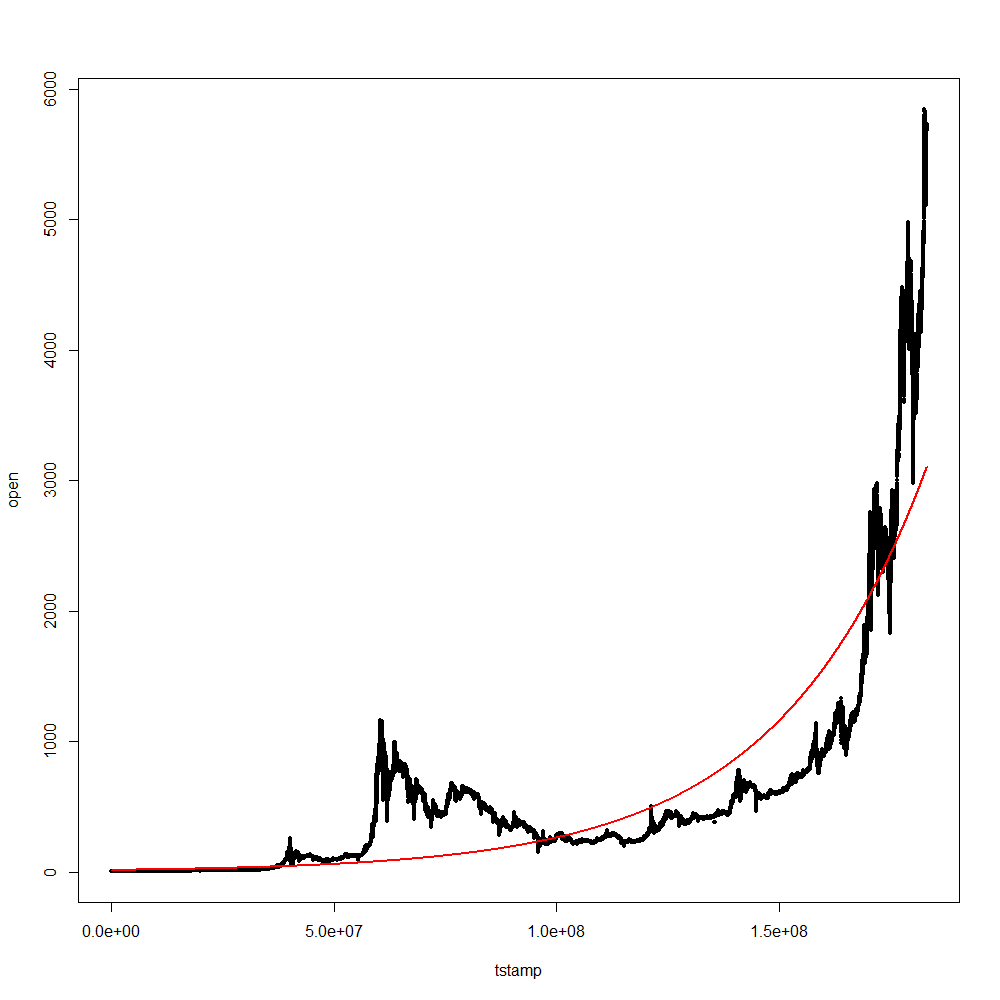
\includegraphics[width=\textwidth]{Exponential.png}
\end{figure}
	
\subsection{Poisson Model Fitting}
The first assumption that was made was that the Poisson Model would have $\lambda$ that would be either near the highest occurring value in the data or the mean. So both the possible values were tried. However, even in the initial run, it was clear that the range of Poisson was not very wide hence trying to fit it further didn't make sense
\begin{Schunk}
\begin{Sinput}
> #Poisson Model for lambda=mean
> btce<-csv2
> par(mfrow=c(1,2))
> hist(btce$Open,freq=FALSE)
> x<-rpois(length(btce[,2]),lambda=mean(btce$Open))
> hist(x,add=TRUE,col=2,freq=FALSE)
> #Poisson model for highest frequency range
> #It appears to be around 250 so we'll give that value a shot
> hist(btce$Open,freq=FALSE)
> x<-rpois(length(btce[,2]),lambda=250)
> hist(x,add=TRUE,col=2,freq=FALSE)
> par(mfrow=c(1,1))
\end{Sinput}
\end{Schunk}
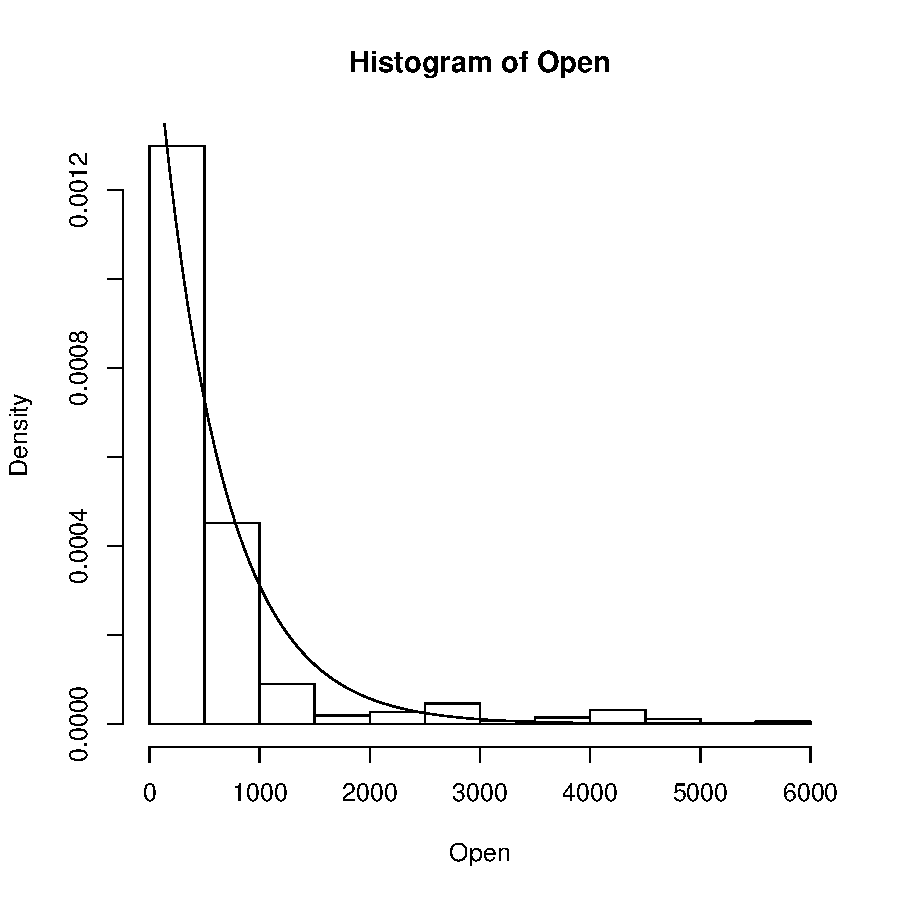
\includegraphics{Report-005}

\subsection{Simulation with Exponential distribution}
After trying to fit the exponential and poisson models to our distribution, we realized that the former seems to fit better compared to the latter. Although we have a peak near the year 2013 which created some residual error but still the error was significantly less compared to others. Hence we chose exponential model to do simulate the bitcoin trading curve.

Let us go through the rationale of doing so. First, we sample the bitstamp dataset for $100000$ random data points and then we plot the density of the same.

\begin{Schunk}
\begin{Sinput}
> bt <- csv2
> NSamples <- 100000
> bts <- bt[sample(length(bt$Timestamp),NSamples),]
> Open <- bts$Open
> # mean of the opening values of the bitcoin
> mean.Open <- mean(Open) 
> # density of the Opening values
> hist(Open, freq= FALSE)   
> # overlaying the exponential curve
> curve(dexp(x,rate=1/mean.Open),add=TRUE,col=2)   
\end{Sinput}
\end{Schunk}
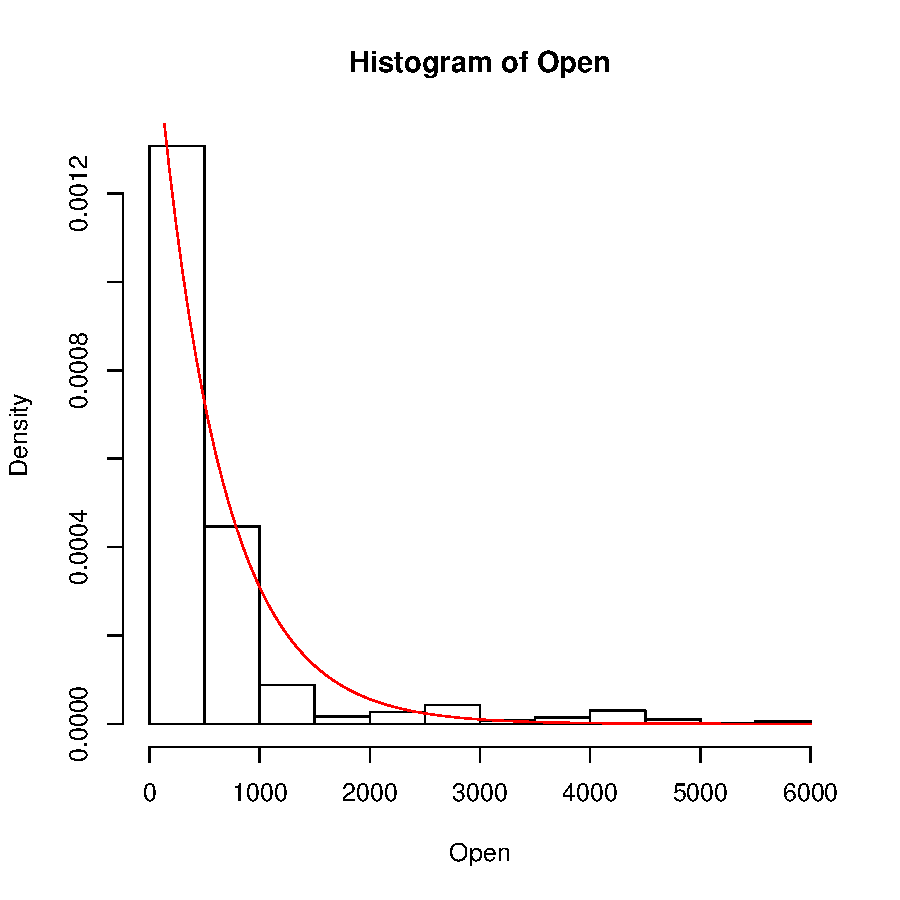
\includegraphics{Report-006}

After plotting the density of the opening values of the dataset, we overlay an exponential density function curve on it. The curve seems to fit fairly well to our dataset and so we finally chose to simulate new sample points for our dataset with an exponential density function.

\begin{Schunk}
\begin{Sinput}
> bt <-csv2
> NSamples <- 100000# number of samples 
> # selecting random sample points
> bts <- bt[sample(length(bt$Timestamp),NSamples),]
> Open <- bts$Open
> # mean of the opening values of the bitcoin
> mean.Open <- mean(Open)     
> # Simulate new observations
> sim.Open <- rexp(NSamples,rate = 1/mean.Open)
> # plotting new observations
> plot(sim.Open~bts$Timestamp,col=4) 
\end{Sinput}
\end{Schunk}

\begin{figure}[H]
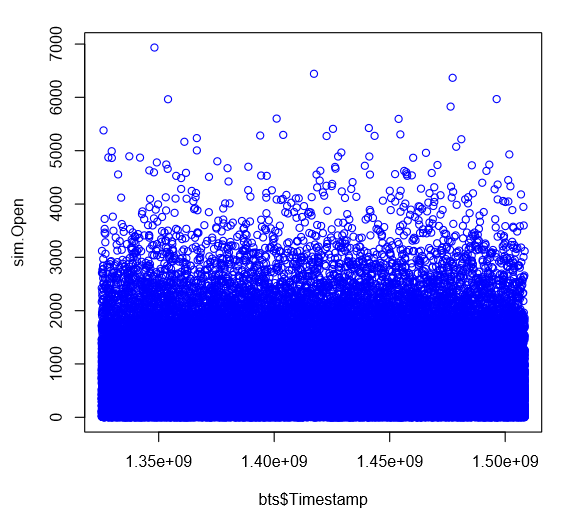
\includegraphics[width=\textwidth]{blue.png}

\label{sampli}
\end{figure}

\begin{Schunk}
\begin{Sinput}
> # density plot of simulated data
> hist(sim.Open,freq = FALSE) 
> # overlaying the exponential curve
> curve(dexp(x,rate=1/mean.Open),add=TRUE,col=2)    
\end{Sinput}
\end{Schunk}
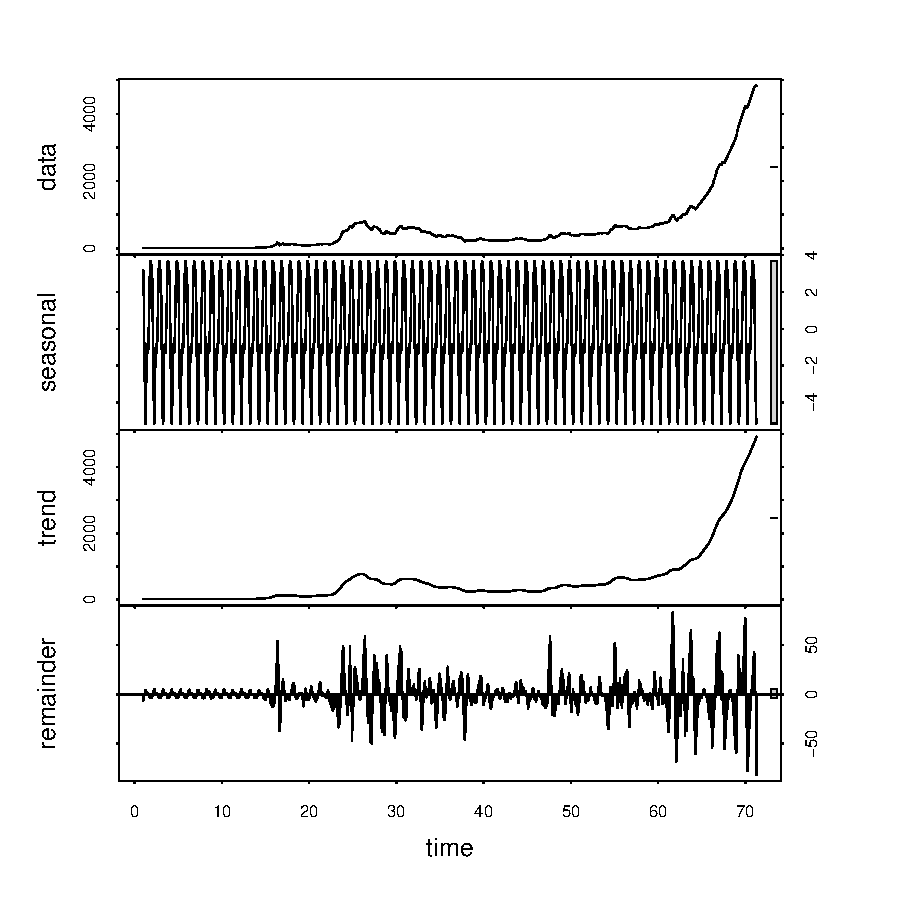
\includegraphics{Report-008}
After simulating with exponential model, we observed that although the histogram of the simulated observations fit exponential curve perfectly, the sample observations seems to random. This is due to the fact that our dataset is a time-series observation while the simulation just create observations which follows a particular probability density function. Hence, we require time-series models for simulating our dataset or forecasting future bitcoin values.

\subsection{Data clustering}
Since our dataset contains a small peak around 2013, so it might be the case that the peaks may belong to different cluster to data. Hence we tried to find the cluster in our dataset using k-means clustering.

\begin{Schunk}
\begin{Sinput}
> ## clusters in dataset
> bt <- csv2
> NSamples <- 100000
> bts <- bt[sample(length(bt$Timestamp),NSamples),]
> par(mfrow=c(2,2))
> # opening times
> xopen <- cbind(TimeStamp = bts$Timestamp, Open = bts$Open)
> cl_open <- kmeans(xopen,2) # find clusters
> plot(xopen,col=cl_open$cluster) # plot the respective clusters
> #closing times
> xclose <- cbind(TimeStamp = bts$Timestamp, Close = bts$Close)
> cl_close <- kmeans(xclose,2) # find clusters
> plot(xclose,col=cl_close$cluster) # plot the respective clusters
> # Low
> xlow <- cbind(TimeStamp = bts$Timestamp, Low = bts$Low)
> cl_low <- kmeans(xlow,2) # find clusters
> plot(xlow,col=cl_low$cluster) # plot the respective clusters
> # High
> xhigh <- cbind(TimeStamp = bts$Timestamp, high = bts$High)
> cl_high <- kmeans(xhigh,2) # obtain clusters
> plot(xhigh,col=cl_high$cluster) # plot the respective clusters
> par(mfrow=c(1,1))
\end{Sinput}
\end{Schunk}
\begin{figure}[H]
\centering
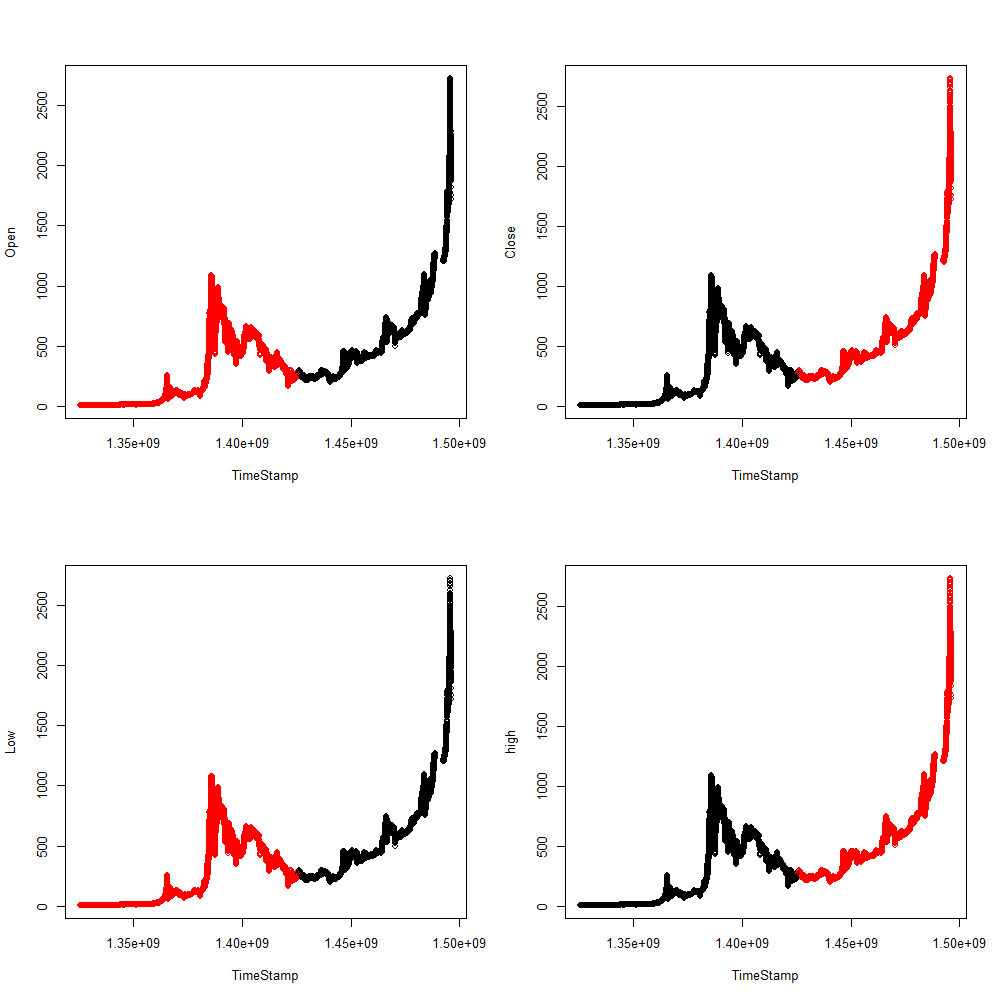
\includegraphics{4plot.png}
\end{figure}

After obtaining the clusters for opening, closing, low and high values of bitcoin we observe that the dataset has can be divided into two clusters, one just at the end of the peak while other containing the exponential growth of bitcoin. Although our data can be divided into two clusters but dividing it and then fitting time-series models to both individually does not seem appropriate. It is because the peak contains some information about the abrupt change in the value of bitcoin affected by external circumstances which is not present in the dataset. Hence fitting models in the two clusters will lead to different models, thereby it would be difficult to draw any inference from the both.

At the end, we decided to do forecasting for the values of bitcoin using an ARIMA model.

%Please add the figures to their related positions according to the word document that I sent on Github for ARIMA model. 
% This is for Who? Didn't we planned to go for R markdown? - Deepak
\section{Forecasting with ARIMA} \label{secARIMA}
%In this report, we explain how to fit an ARIMA model to our data (Bitcoin Opening Values) using R. - This line is not required - Deepak
ARIMA models have a reputation for being transformative and employing historical data for predictions. Here, we will fit a model to our Bitcoin data so that we will be able to do forecasting for future values of bitcoin. 
\subsection{Introduction to ARIMA}
ARIMA is the abbreviation for auto-regressive integrated moving average and its main components are ($P$, $d$, $q$) parameters.

The \textbf{auto regressive} ($AR(p)$) component is referring to the use of past values in the regression equation for the output series. The auto-regressive parameter $p$ specifies the number of lags used in the model. 

The $d$ represents the degree of differencing in the \textbf{integrated} ($I(d)$) component. Differencing a series involves simply subtracting its current from previous values d times.

A \textbf{moving average} ($MA(q)$) component represents the error of the model as a combination of previous error terms $e_t$.
 
Differencing, autoregressive, and moving average components make up a non-seasonal ARIMA model which can be written as a linear equation:

\begin{equation}
Y_t=c+\phi_1 y_(d t-1)+\phi_p y_(d t-p)+...+\theta_1 e_(t-1)+\theta_q e_(t-q)+e_t
\end{equation}

where $y_d$ is $Y$ differenced $d$ times and $c$ is a constant.

\subsection{ARIMA model limitations}
These models are suitable for long and robust series where the present values are dependent on the past values.
 
\subsection{Outline}
In order to fit a model to our data using ARIMA, here is the outline of what we need to do:
\begin{itemize}
\item \textbf{Data Examination:}
\begin{itemize}
\item Plotting the data in order to find patterns and irregularities
\item Dropping the missing values and outliers (tsclean() is a suitable method for this purpose)
\item Calculating the logarithm of the time series to see a growth trend
\end{itemize}
\item \textbf{Data Analyzing:}
\begin{itemize}
\item Finding trends or seasonality in the data if there is any
\item Applying $decompose()$ or $stl()$ for removing the components of the series
\end{itemize}
\item \textbf{Stationarity}
\begin{itemize}
\item Is there any stationarity in the data?
\item Use adf.test(), ACF, PACF plots to determine order of differencing needed
\end{itemize}
\item Autocorrelations and selecting model order
\begin{itemize}
\item Finding out the order of ARIMA using ACF() and PACF() plots
\end{itemize}
\item \textbf{Fit an ARIMA model}
\item \textbf{Assess and repeat}
\begin{itemize}
\item Examine the  residuals to make sure there is no pattern and they are normally distributed
\item In case of existing any visible patterns, draw ACF/ PACF plots to figure out if any additional parameters is needed.
\item Refit model if it is necessary. Testing model errors and fit criteria such as AIC or BIC.
\item Compute fitting model by means of the selected model.
\end{itemize}
\end{itemize}

\subsection{How to fit a model using ARIMA - Description}
\subsubsection*{Step 1: Load R packages}

In this study for fitting ARIMA model, we will be using the following libraries. Moreover, we will be utilizing ``bitstampUSD_1-min_data_2012-01-01_to_2017-10-20'' file as our dataset.
\begin{Schunk}
\begin{Sinput}
> #install.packages("tseries","forecast","ggplot2")
> library('ggplot2')
> library('forecast')
> library('tseries')
> btc<-csv
\end{Sinput}
\end{Schunk}
\subsubsection*{Step 2: Data Cleaning}
Since our dataset contains too many Nan values, we will be using a method to replace them with their closest values. Then, we changed the intervals of the Bitcoin opening values from minute to day to make our data more visually appealing. Furthermore, we transformed the timestamp to date.
\begin{Schunk}
\begin{Sinput}
> #Replacing the Nan opening values with the nearest values 
> replaceNanNearst <- function(dat) {
+   N <- length(dat)
+   na.pos <- which(is.na(dat))
+   if (length(na.pos) %in% c(0, N)) {
+     return(dat)
+   }
+   non.na.pos <- which(!is.na(dat))
+   intervals  <- findInterval(na.pos, non.na.pos,
+                              all.inside = TRUE)
+   left.pos   <- non.na.pos[pmax(1, intervals)]
+   right.pos  <- non.na.pos[pmin(N, intervals+1)]
+   left.dist  <- na.pos - left.pos
+   right.dist <- right.pos - na.pos
+ 
+   dat[na.pos] <- ifelse(left.dist <= right.dist,
+                         dat[left.pos], dat[right.pos])
+   return(dat)
+ }
> btc$openC<-replaceNanNearst(btc$Open)
> #Changing the interval from minute to minute to day to day
> sq<-seq(1,length(btc$openC),by = 1440)
> btc_date<-btc$Timestamp[sq]
> BTC<- data.frame(btc_open=btc$openC[sq],
+                  btc_Date=as.Date(as.POSIXct(btc_date,
+                                              origin = "1970-01-01",
+                                              tz = "GMT")))
\end{Sinput}
\end{Schunk}
\subsubsection*{Step 3: Analyzing the data}
Plotting the data to find the outliers and irregularities is of importance.
\begin{Schunk}
\begin{Sinput}
> #Analyzing the data
> ggplot(BTC, aes(btc_Date, btc_open))+ 
+   geom_line() + scale_x_date("Year")+ 
+   ylab("Daily bitcoin openning value")+
+   xlab("Year")
\end{Sinput}
\end{Schunk}
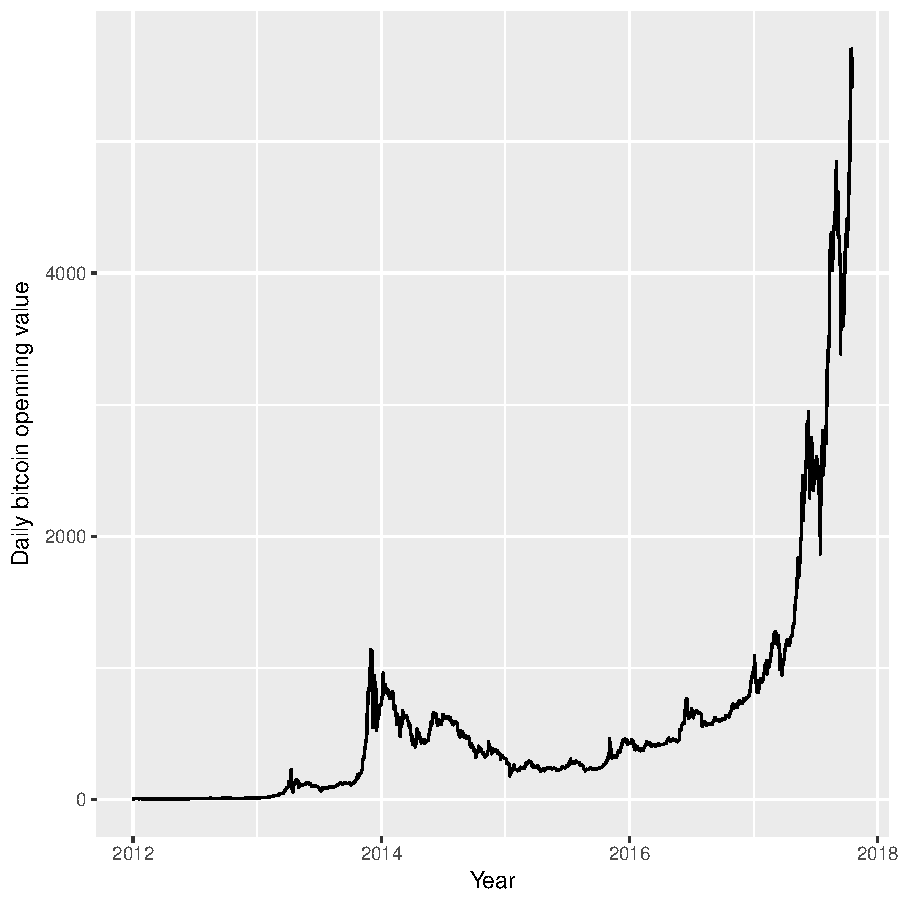
\includegraphics{Report-012}

In some cases, the opening value of Bitcoin increased to 1125 USD on month and dropped to 500 USD the next month. These are doubted outliers that might incline the model by deviating the summaries. Tsclean() in R provides facilities for passing up these outliers. This method replaces outliers applying series smoothing and decomposition. For this purpose, first a time series object should be created using $ts()$ command to be passed to $tsclean()$:

Plotting the clean series using ggplot:

\begin{Schunk}
\begin{Sinput}
> #Removing the outliers
> count_ts = ts(BTC[, c('btc_open')])
> BTC$clean_open = tsclean(count_ts)
> ggplot() +
+ geom_line(data = BTC, aes(x = btc_Date, y = clean_open))+
+   ylab("Daily bitcoin opening value")
\end{Sinput}
\end{Schunk}
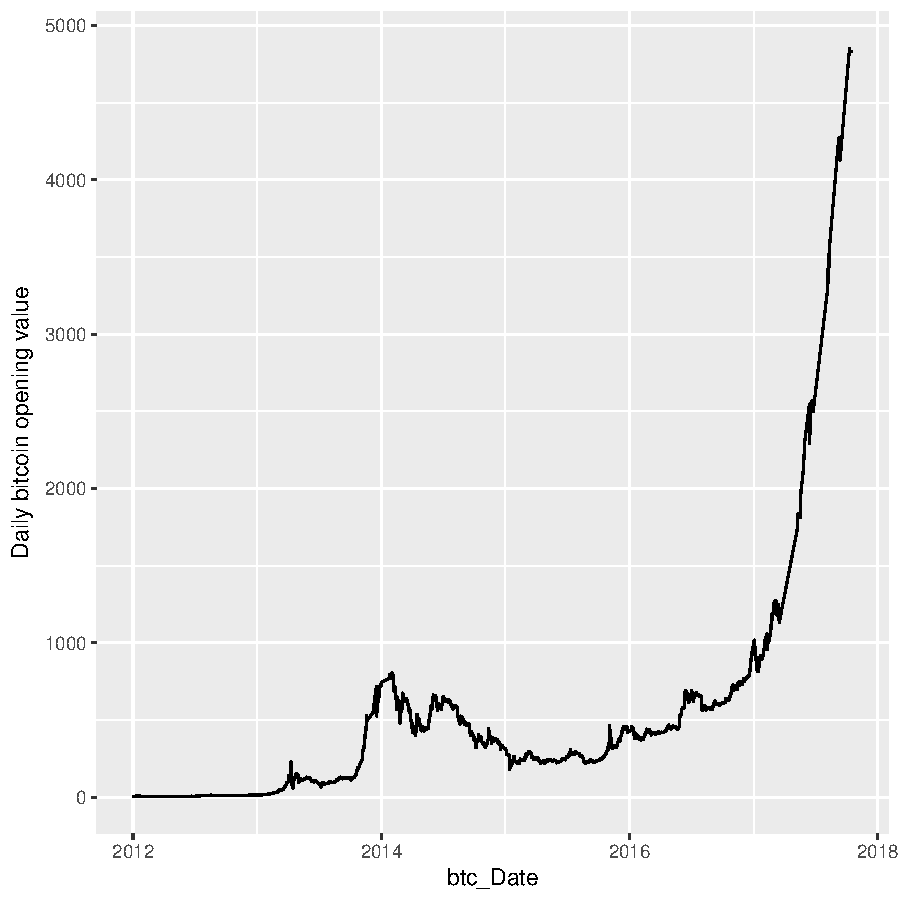
\includegraphics{Report-013}

It is noticeable that even after ignoring the outliers, there are still fluctuations in the Bitcoin opening values. One of the promising solutions to this issue is through considering a line connecting its bigger bottoms and peaks when smoothing the fluctuations. This concept is known as moving average in time series. This meaning calculates the average of the points across different intervals and therefore makes the data a more predictable series. 
A moving average (MA) of order m can be calculated using the following formula:
\[
MA=1/m \sum_{j}^{k}-k^(y_t+j) 
\]
Where $y$ is the series, $k$ is the number of periods around each point and $m=2k+1$.
It is worth noting that the moving average here is completely different from the $MA(q)$ component in the definition of ARIMA. $MA(q)$ is related to error lags but the summary statistic of moving average is a part of the data smoothing technique.

We have a smoother function as we expand the size of the window for the moving average. If we take monthly ( or seasonally) instead of weekly moving average, we can have a more predictable series.
\begin{Schunk}
\begin{Sinput}
> #Making the clean data(The data with no outliers) smoother using the moving average
> BTC$open_ma = ma(BTC$clean_open, order=7) 
> BTC$open_ma30 = ma(BTC$clean_open, order=30)
> BTC$open_ma120 = ma(BTC$clean_open, order=120)
> ggplot() +
+   geom_line(data = BTC, aes(x = btc_Date, 
+                             y = clean_open, colour = "real data")) +
+   geom_line(data = BTC, aes(x = btc_Date, 
+                             y = open_ma,   colour = "Weekly Moving Average"))+
+   geom_line(data = BTC, aes(x = btc_Date, 
+                             y = open_ma30, colour = "Monthly Moving Average"))+
+   geom_line(data = BTC, aes(x = btc_Date, 
+                             y = open_ma120, colour = "Seasonal Moving Average"))+
+   xlab("Date")+
+   ylab("Bitcoin opening value")
\end{Sinput}
\end{Schunk}
\begin{figure}[H]
\begin{center}
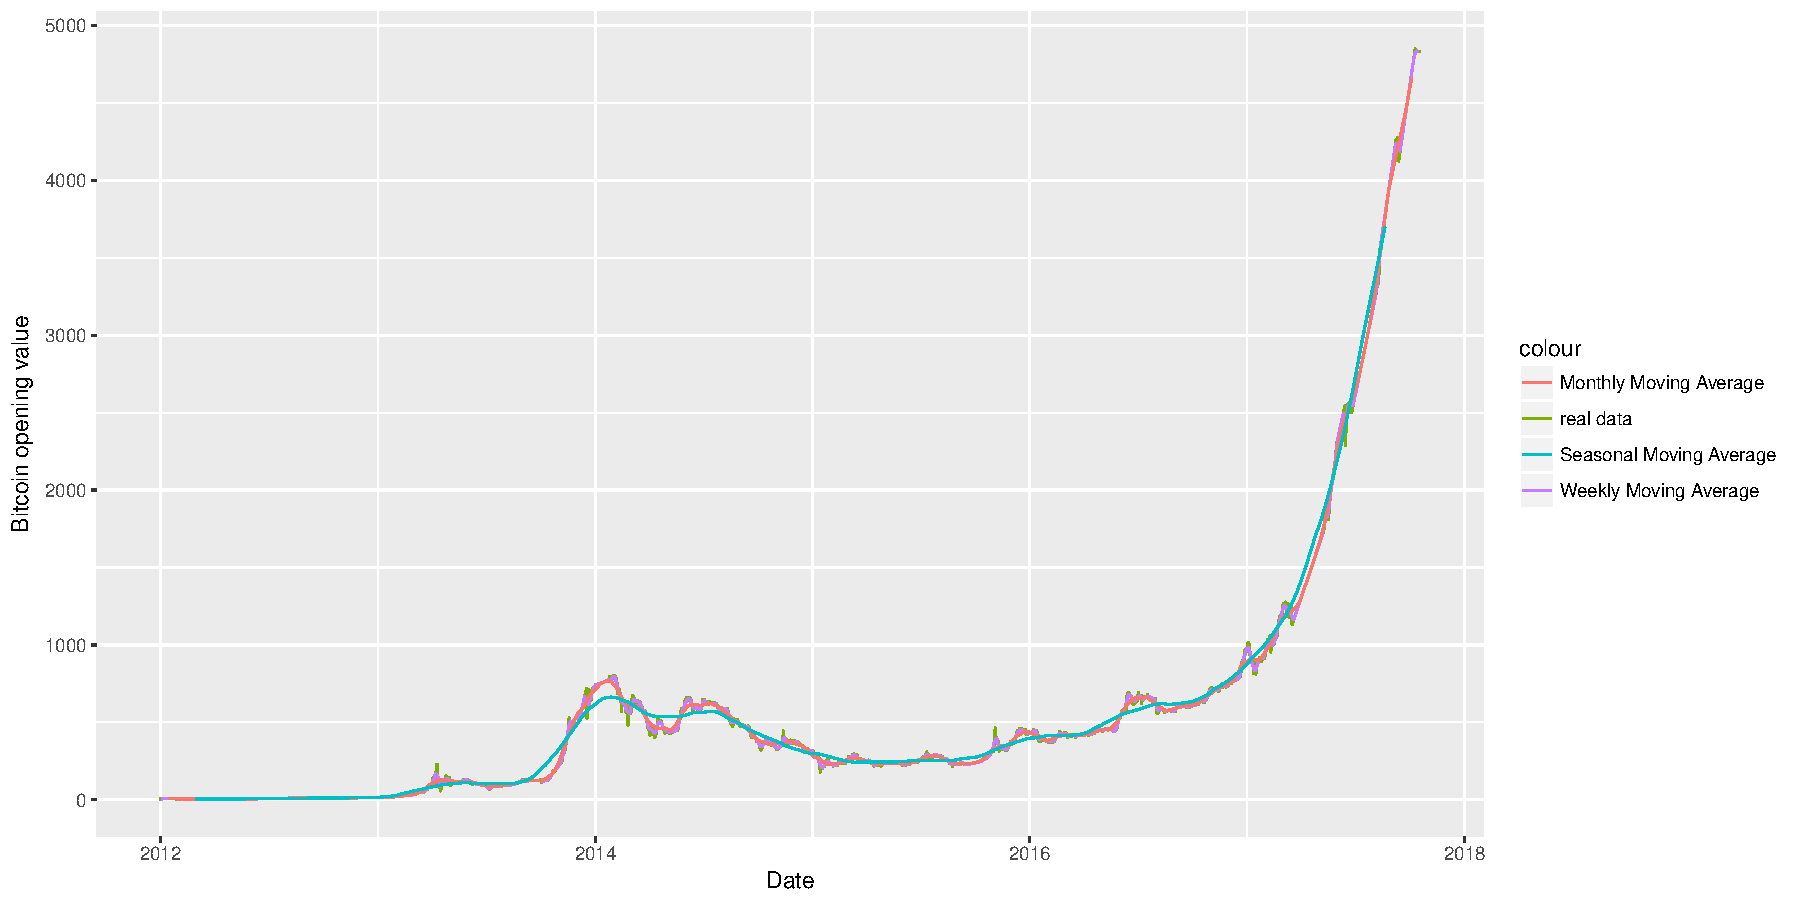
\includegraphics[width=\textwidth,totalheight=0.6\textwidth]{Report-arima}
\end{center}
\label{arima}
\end{figure}
As can be seen, the Seasonal Moving Average offers the smoothest data and we will model it (as shown by green line above) for simplicity. 

\subsubsection*{Step 4: Decompose the data}

The corner stones for analyzing a time series are seasonality, trend and cycle. These components detect the historical patterns of the series. In case of being available, these components can contribute in analyzing the behavior of the series in order to be able to create a forecasting model.

Seasonal component is related to the fluctuations in the data in seasonal cycles. For example, in which seasons, the Bitcoin value is larger and in which seasons in has smaller values.
Trend component is assigned to the whole pattern of the series. Does the series have an increasing or decreasing trend over all of the intervals?

Cycle component is about all of the increasing or decreasing trends that are not seasonal. In general, trend and cycle components are considered together as one.
The last part of the series that cannot be referred to any of the other components is called residual or error.

The process of taking out these components is called decomposition. 

For example, if Y is the Bitcoin opening value, we can decompose the series by applying an additive or multiplicative model:
\begin{equation}
Y=S_t*T_t*E_t
\end{equation}
Where $S$, $T$ and $E$ are seasonal, trend and error components, respectively.

An additive model is more appropriate for the conditions that seasonal or trend components are not proportional to the level of series. In these situations, we can just overlay the components together to rebuild the series. In contrast, if the seasonality is dependent to trend of the series, a multiplicative model can be more efficient.

As fitting a model to seasonal data is a complicated process, we will explain how to de-seasonalize the series and use a "vanilla" non-seasonal ARIMA model.
In order to do this, we first calculate seasonal component of the data using $stl()$. The $Stl()$ is a function for decomposing and forecasting the series. It calculates the seasonal component of the series using smoothing, and configuring the series by subtracting seasonality.
  
\begin{Schunk}
\begin{Sinput}
> #Decomposion
> count_ma = ts(na.omit(BTC$open_ma), frequency=30)
> decomp = stl(count_ma, s.window="periodic")
> deseasonal_open <- seasadj(decomp)
> plot(decomp)
\end{Sinput}
\end{Schunk}
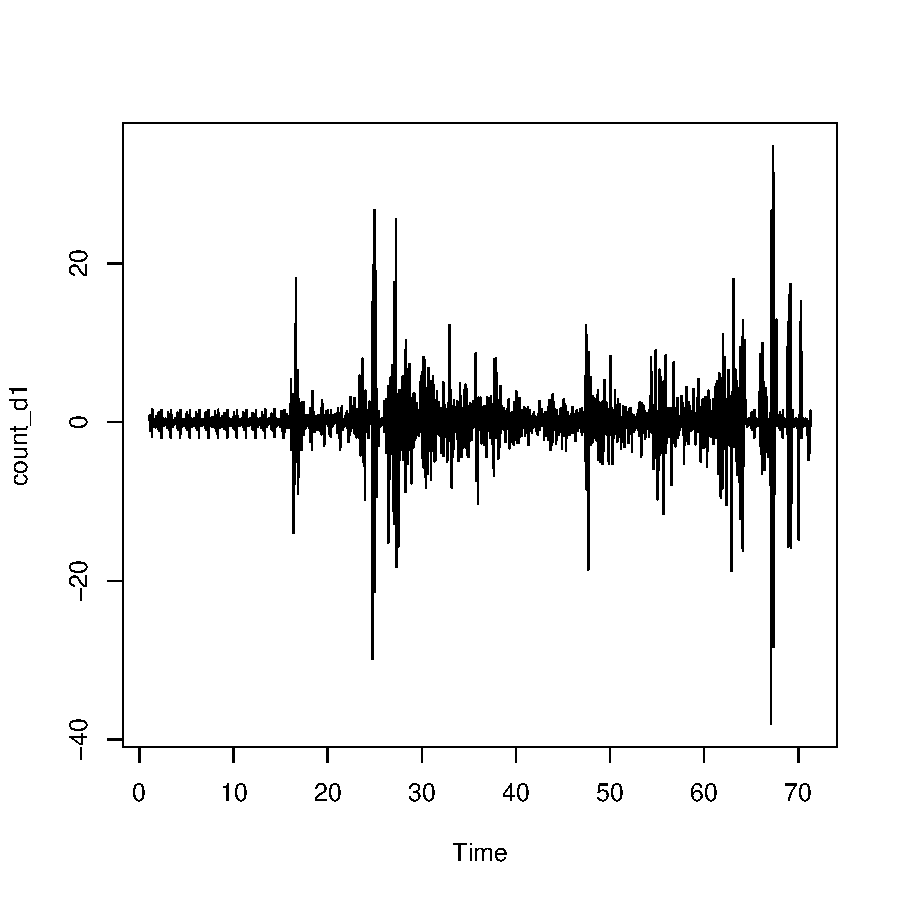
\includegraphics{Report-015}
$Seasadj()$ is a method for removing the seasonality. We set the periodicity of the data (i.e., the number of observations per period) for the frequency parameter in $ts()$ object. As we utilize smoothed daily data, we have 30 observations per month.

\subsubsection*{Step 5: Stationarity}

Fitting an ARIMA model requires series to be stationary which means that its mean, variance and autocovariance are independent from time. One of the formal statistical tests for stationarity is the augmented Dickey-Fuller (ADF). The null hypothesis here is that the series is non-stationary. ADF checks if the change in the Y values can be described by lagged value and a linear trend. If values of Y are related to lagged values and a trend component emerges, the series is considered to be non-stationary and null hypothesis will not be rejected.
\begin{Schunk}
\begin{Sinput}
> #ADF Test for testing stationarity
> adf.test(count_ma, alternative = "stationary")
\end{Sinput}
\begin{Soutput}
	Augmented Dickey-Fuller Test

data:  count_ma
Dickey-Fuller = 5, Lag order = 12, p-value = 0.99
alternative hypothesis: stationary
\end{Soutput}
\end{Schunk}
The opening values of Bitcoin are non-stationary. The average of opening values of Bitcoin change through time. The ADF test does not reject the NULL hypothesis and corroborates our guess.
The non-stationary series can be transformed to stationary ones by deducting one period's values from the previous period's values. Differencing can assist in deleting the trends or cycles from the data and makes it stationary:
\begin{equation}
Y_(d_t )=Y_t-Y_(t-1)
\end{equation}
In a similar vein, differencing can be used for removing seasonal patterns at specific lags:
\begin{equation}
Y_(d_t )=(Y_t-Y_(t-s) )-(Y_(t-1)-Y_(t-s-1))
\end{equation}
where $d$ component of ARIMA represents the number of carried out differences.

\subsubsection*{Step 6: Autocorrelations and Choosing Model Order}

In this section, the methods for choosing the order of differencing will be explained. Auto Correlation Function (ACF) is an efficient method for determining if a series is stationary. It is also beneficial in choosing the order of the parameters of the ARIMA model.  In case of existing a correlation between a variable and its lags, there are some trends and therefore, the series changes over time. 

ACF plots show the correlation between a series and its lags. Partial autocorrelation plots (PACF) show the correlation between a variable and its lags that is not included by previous lags. 
As can be seen, there are autocorrelations with many lags in Bitcoin opening values by the ACF plot. This is because of the carry-over correlation from the early lags. However, the PACF plot does not show any spikes.

\begin{Schunk}
\begin{Sinput}
> #Plotting ACF and PACF plots for
> #displaying the auto correlation
> Acf(count_ma, main='')
> Pacf(count_ma, main='')
\end{Sinput}
\end{Schunk}
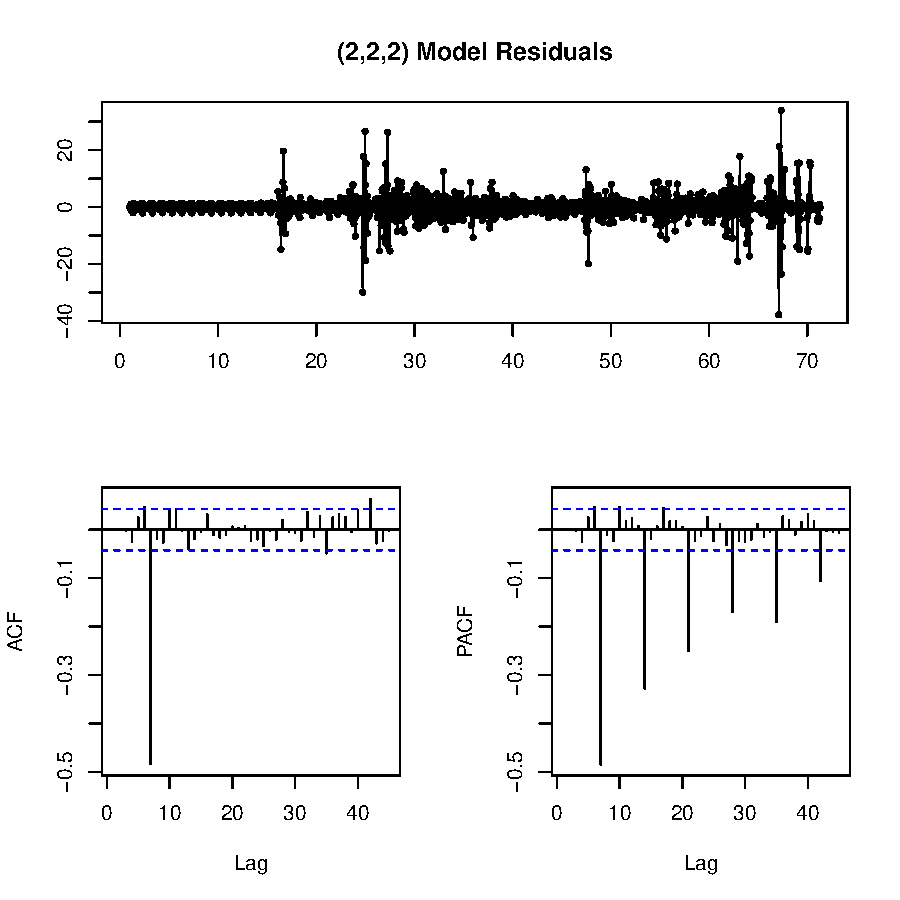
\includegraphics{Report-017}

We will start from $d=1$ and reevaluate if more differencing is needed. The null hypothesis of being non-stationary is rejected with the $adf$ test. Considering the plotted differenced series, there is an oscillating pattern around $0$ with no visible strong trend. Therefore, differencing of order $1$ terms seems to be sufficient but differencing of order $2$ decreases the number spikes in ACF so it should be included in the model. 

\begin{Schunk}
\begin{Sinput}
> #Plotting the differenced series for choosing the order of differencing
> count_d1 = diff(deseasonal_open, differences = 2)
> plot(count_d1)
> adf.test(count_d1, alternative = "stationary")
\end{Sinput}
\begin{Soutput}
	Augmented Dickey-Fuller Test

data:  count_d1
Dickey-Fuller = -14.023, Lag order = 12, p-value = 0.01
alternative hypothesis: stationary
\end{Soutput}
\end{Schunk}
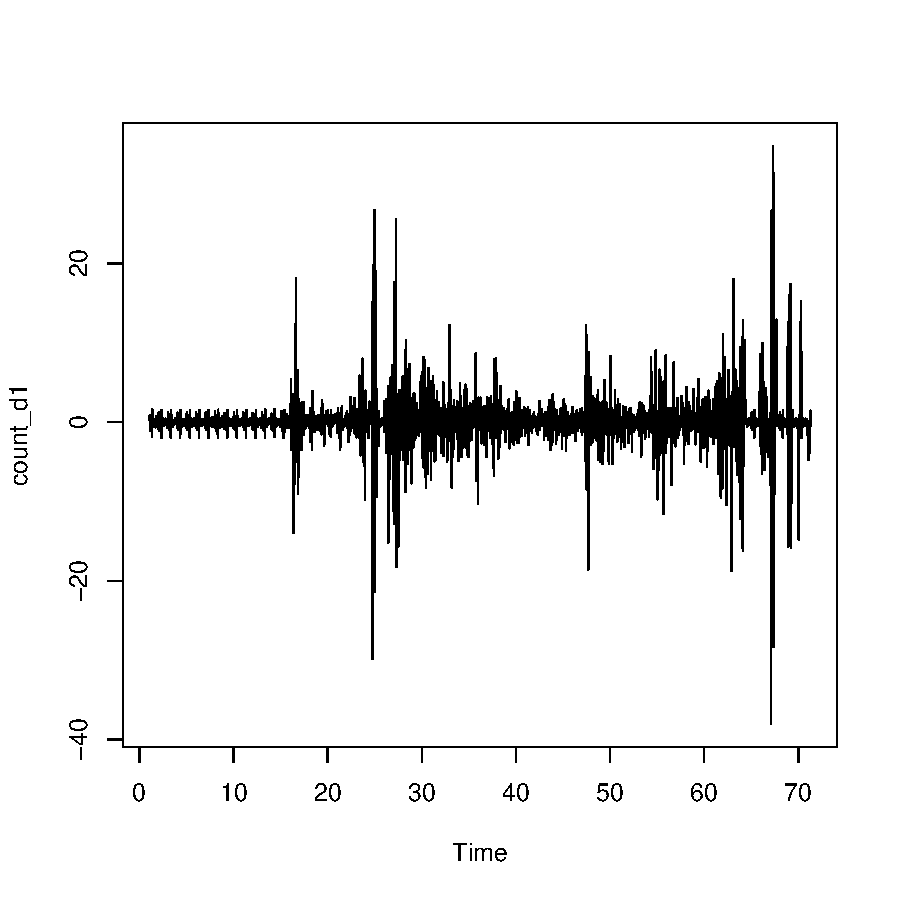
\includegraphics{Report-018}


Next, spikes at particular lags of the differenced series could be of benefit when it comes to choosing the p or q for our model:
\begin{Schunk}
\begin{Sinput}
> #Plotting ACF and PACF plots of the differencing 
> #series to choose p and q for the model
> Acf(count_d1, main='ACF for Differenced Series')
> Pacf(count_d1, main='PACF for Differenced Series')
\end{Sinput}
\end{Schunk}
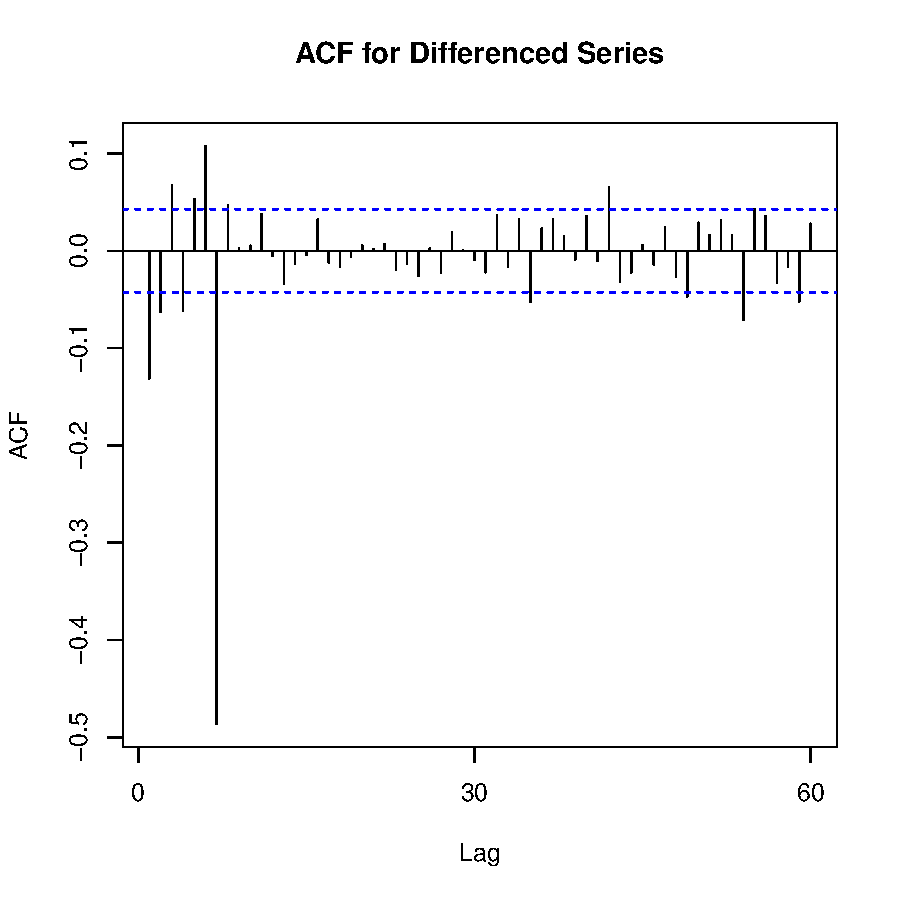
\includegraphics{Report-019}


There are noticeable auto correlations at lag1, 2 and 7. In PACF plot, there are significant spikes at lag 1, 2 and 7 and 14. Therefore, we would test models with AR or MA components of order 1, 2, 7 or 14. A spike at lag 7 and 14 may imply that there is a seasonal pattern available, perhaps as day of the week. 

\subsubsection*{Step 7: Fitting an ARIMA model}

We should use the forecast package to apply the $arima()$ function for determining order of the model. We can also automatically specify a set of optimal ($p$, $d$, $q$) using $auto.arima()$.This function searches through combinations of order parameters and picks the set that optimizes model fit criteria.

There are some criteria for evaluating the quality of fitting models. Among the most reputable ones, we can mention Akaike information criteria (AIC) and Baysian information criteria (BIC). These criteria can examine the amount of information lost for the chosen model. The objective here is that the selected minimizes AIC and BIC.

For applying $auto.arima()$, it is necessary to complete steps 1-5 to comprehend the series and analyzing model results. We can also determine maximum order of ($p$, $d$, $q$) using $auto.arima()$ that  is by default equal to $5$.
\begin{Schunk}
\begin{Sinput}
> #Fitting the model
> auto.arima(deseasonal_open, seasonal=FALSE)
\end{Sinput}
\begin{Soutput}
Series: deseasonal_open 
ARIMA(0,2,3) 

Coefficients:
          ma1      ma2     ma3
      -0.1378  -0.0582  0.0670
s.e.   0.0218   0.0212  0.0239

sigma^2 estimated as 11.82:  log likelihood=-5592.87
AIC=11193.75   AICc=11193.76   BIC=11216.36
\end{Soutput}
\end{Schunk}

The offered parameters ($2$, $2$, $2$) by the automated procedure are compatible with our expectations from the explained steps. The model incorporates differencing of degree 2, and applies an autoregressive term of the second lag and a moving average model of order 2.

Our model regarding the ARIMA notation can be defined as follows:
\begin{equation}
\tilde{Y}_{d_t}=0.551Y_{t-1}-0.2496e_{t-1}+E
\end{equation}

Here, $E$ is some error and the original series is differenced with order 2.

\subsubsection*{Step 8: Evaluate and Iterate}

So far, we fitted a model to our data that can be used for forecasting, but how much we can trust it? For this purpose, we can test ACF and PACF plots for model residuals.  In case of correctly selecting model order parameters and structure, there should not be any significant autocorrelations.

\begin{Schunk}
\begin{Sinput}
> #Testing the model using model residuals
> fit<-auto.arima(deseasonal_open, seasonal=FALSE)
> tsdisplay(residuals(fit), lag.max=45, main='(2,2,2) Model Residuals')
\end{Sinput}
\end{Schunk}
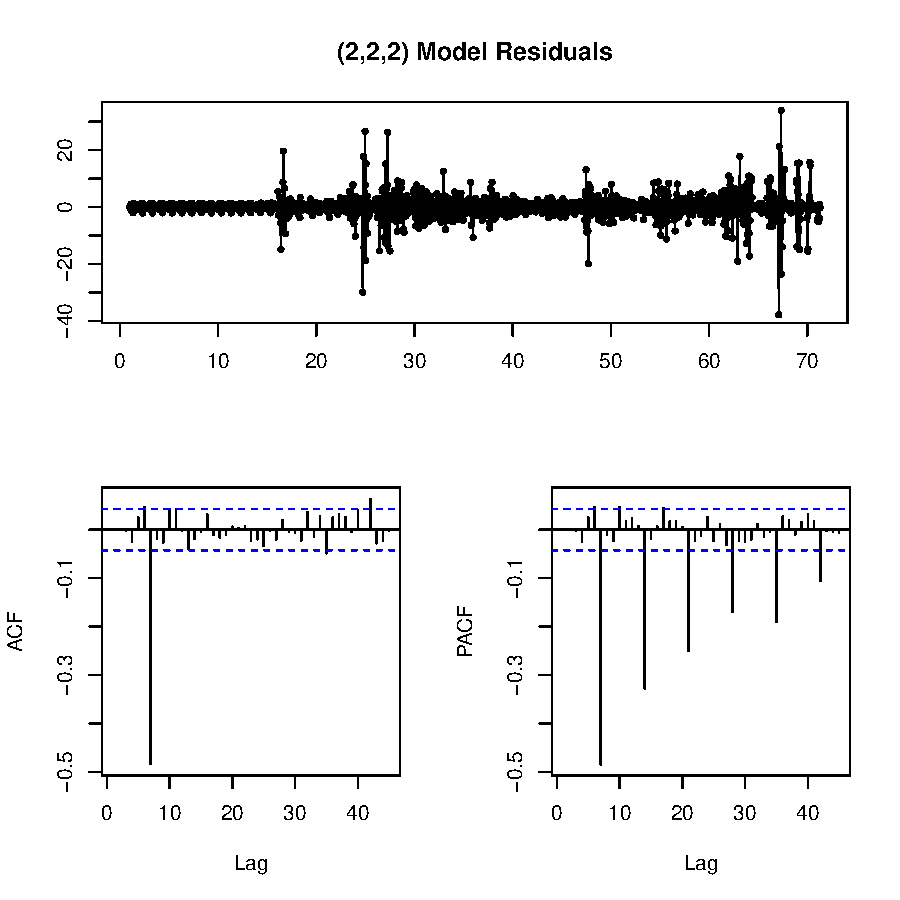
\includegraphics{Report-021}
From the $ACF$/$PACF$ and model residuals plots , we can see that there is a repeating pattern repeating at lag 7. This suggests that our model might work better with a different configuration, such as $p = 7$ or $q = 7$. 

We can do the fitting process from the beginning for $MA(7)$ and test the model again. In the new model, there are no observable autocorrelations. In case of being correctly selected, the model does not show any patterns in the model residuals. If the residuals are normally distributed, it means that the model correctly fits the series. Tsdisplay() function is applicable in this situation. Residuals plots display a smaller error range, more or less centered around 0. As can be seen, the AIC is smaller when we select ($2$,$2$, $7$) for the parameters.

\begin{Schunk}
\begin{Sinput}
> #Fitting the model with new parameters
> fit2 = arima(deseasonal_open, order=c(2,2,7))
> tsdisplay(residuals(fit2), lag.max=15, main='Seasonal Model Residuals')
> arima(x = deseasonal_open, order = c(2, 2, 7))
\end{Sinput}
\begin{Soutput}
Call:
arima(x = deseasonal_open, order = c(2, 2, 7))

Coefficients:
          ar1      ar2     ma1     ma2     ma3     ma4     ma5     ma6      ma7
      -0.1560  -0.0877  0.0229  0.0274  0.0315  0.0308  0.0211  0.0318  -0.9671
s.e.   0.0227   0.0226  0.0079  0.0076  0.0073  0.0076  0.0075  0.0079   0.0077

sigma^2 estimated as 6.223:  log likelihood = -4933.61,  aic = 9887.22
\end{Soutput}
\end{Schunk}
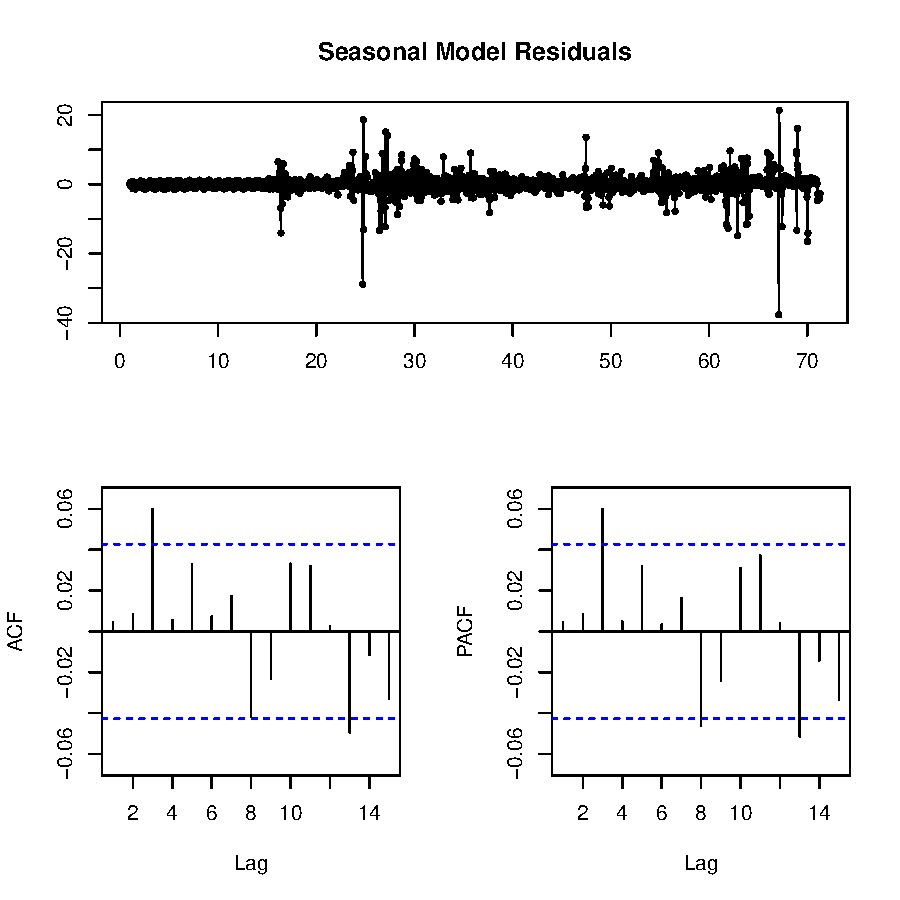
\includegraphics{Report-022}

It is easy to do the prediction by a fitted model in R. We just need to determine forecast horizon h periods ahead for making the predictions.
\begin{Schunk}
\begin{Sinput}
> #Forecasting
> fcast <- forecast(fit2, h=30)
> plot(fcast)
\end{Sinput}
\end{Schunk}
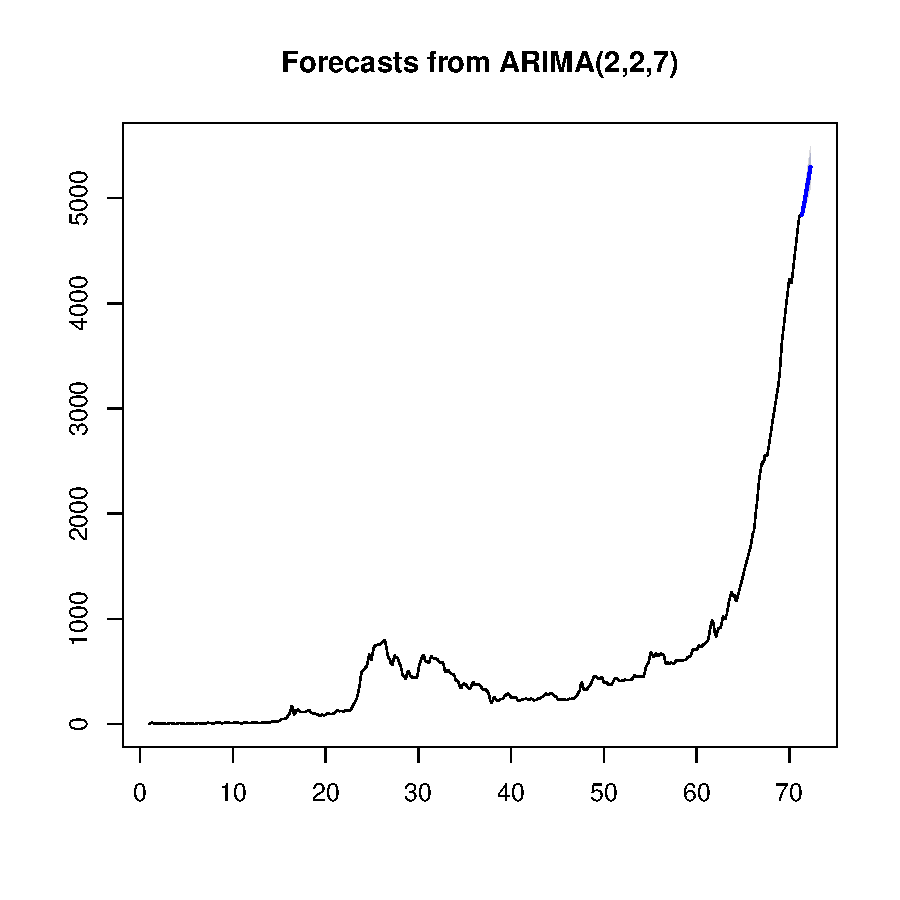
\includegraphics{Report-023}

In order to find out how the model will work in future, we can fit the model to a part of the data (hold-out set) and then compare the forecast with the actual values. 
\begin{Schunk}
\begin{Sinput}
> #Testing the performance of the model
> hold <- window(ts(deseasonal_open), start=1734)
> fit_no_holdout = arima(ts(deseasonal_open[-c(1734:1764)]), order=c(2,2,7))
> fcast_no_holdout <- forecast(fit_no_holdout,h=30)
> plot(fcast_no_holdout, main=" ")
> lines(ts(deseasonal_open))
\end{Sinput}
\end{Schunk}
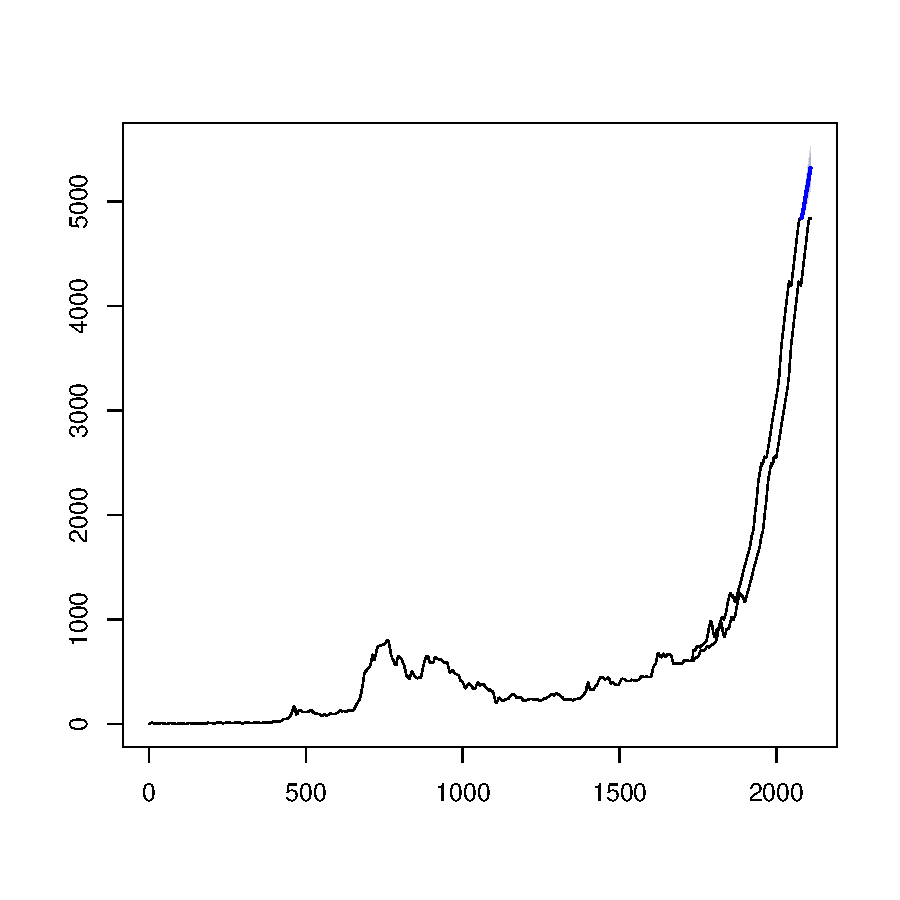
\includegraphics{Report-024}

The blue line that shows forecast has an upward trend which shows the same behavior as the series. This model can be used as a benchmark against more complicated models.
Forecasting improvement  
We can improve the forecast by adding back the seasonal component to the model or by setting ($P$, $D$, $Q$) components in the auto.arima() function. 
\begin{Schunk}
\begin{Sinput}
> #Forecasting improvement
>  fit_w_seasonality = auto.arima(deseasonal_open, seasonal=TRUE)
>  fit_w_seasonality
\end{Sinput}
\begin{Soutput}
Series: deseasonal_open 
ARIMA(0,2,3) 

Coefficients:
          ma1      ma2     ma3
      -0.1378  -0.0582  0.0670
s.e.   0.0218   0.0212  0.0239

sigma^2 estimated as 11.82:  log likelihood=-5592.87
AIC=11193.75   AICc=11193.76   BIC=11216.36
\end{Soutput}
\begin{Sinput}
>  seas_fcast <- forecast(fit_w_seasonality, h=30)
>  plot(seas_fcast)
\end{Sinput}
\end{Schunk}
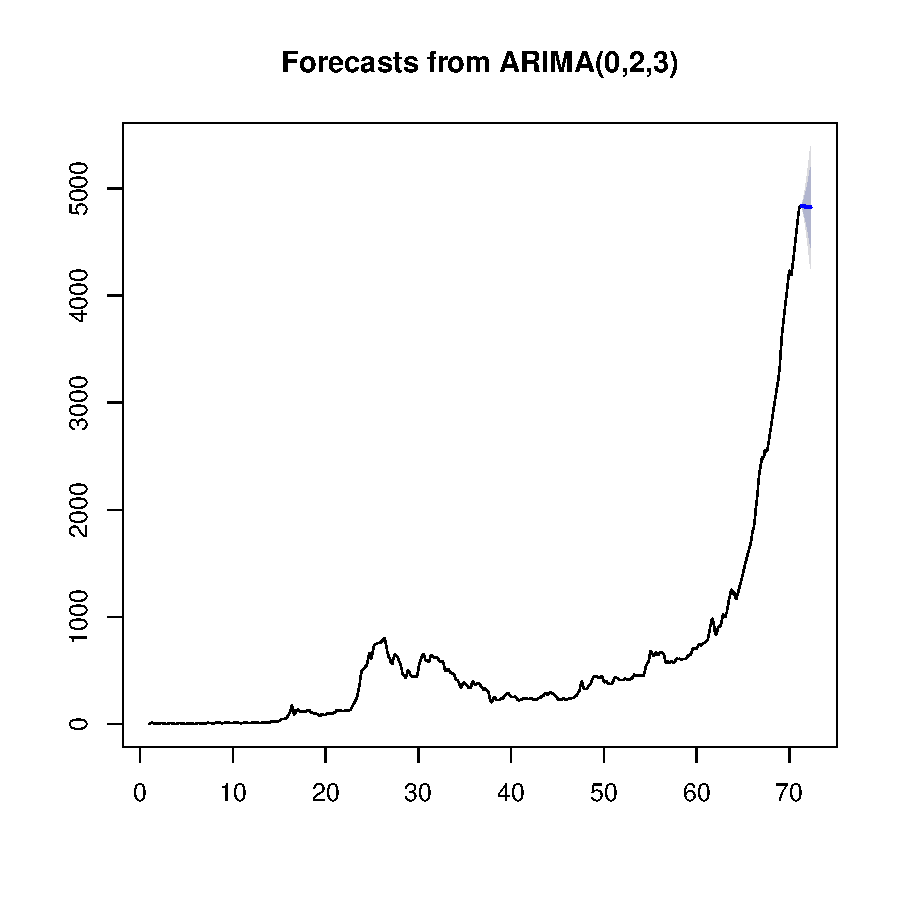
\includegraphics{Report-025}

The 80\% and 95\% confidence limits are shown with the darker and lighter grey respectively. It is inevitable that long-run forecasts cause a high level of uncertainty. This is due to the current value of Y is dependent on previous ones.
We can evaluate the model residuals again. As shown, the autocorrelation with lag 7 recommends a higher order component for the model.

It should be noted that we followed the tutorial to fit the ARIMA model to our data. 

\section{Conclusions}


\end{document}
